\documentclass{article}
\usepackage{amsmath}
\usepackage{enumitem}
\usepackage{listings}
\usepackage{color}
\usepackage{graphicx}
\usepackage[left=2cm, right=2cm, top=3cm]{geometry}
\usepackage{enumitem}
\usepackage{hyperref,theoremref}
\hypersetup{
	pdftitle={Waves Homework Set 5},
	colorlinks=true, linkcolor=doc!90,
	bookmarksnumbered=true,
	bookmarksopen=true
	pdfauthor={Víctor Mira Ramírez}
	pdfpagemode=FullScreen
}
\usepackage[most,many,breakable]{tcolorbox}
\usepackage{xcolor}
\usepackage{varwidth}
\usepackage{varwidth}
\usepackage{etoolbox}
\usepackage{tikz-cd}
\usepackage{titlesec}
\titleformat{\section}{\normalfont\fontsize{17.28pt}{12pt}\selectfont\bfseries}{\thesection}{1em}{}

\newcommand{\pregunta}[1]{\begin{note}#1\end{note}}
\usetikzlibrary{arrows,calc,shadows.blur}
\tcbuselibrary{skins}
\newtcolorbox{note}[1][]{%
	enhanced jigsaw,
	colback=gray!10!white,%
	colframe=gray!80!black,
	size=small,
	boxrule=1pt,
	title=\textbf{Question:},
	halign title=flush center,
	coltitle=black,
	drop shadow=black!50!white,
	attach boxed title to top left={xshift=1cm,yshift=-\tcboxedtitleheight/2,yshifttext=-\tcboxedtitleheight/2},
	minipage boxed title=2.5cm,
	boxed title style={%
			colback=white,
			size=fbox,
			boxrule=1pt,
			boxsep=2pt,
			underlay={%
					\coordinate (dotA) at ($(interior.west) + (-0.5pt,0)$);
					\coordinate (dotB) at ($(interior.east) + (0.5pt,0)$);
					\begin{scope}[gray!80!black]
						\fill (dotA) circle (2pt);
						\fill (dotB) circle (2pt);
					\end{scope}
				},
		},
	#1,
}
\definecolor{dkgreen}{rgb}{0,0.6,0}
\definecolor{gray}{rgb}{0.5,0.5,0.5}
\definecolor{mauve}{rgb}{0.58,0,0.82}

\lstset{frame=tb,
  language=Python,
  aboveskip=3mm,
  belowskip=3mm,
  showstringspaces=false,
  columns=flexible,
  basicstyle={\small\ttfamily},
  numbers=none,
  numberstyle=\tiny\color{gray},
  keywordstyle=\color{blue},
  commentstyle=\color{dkgreen},
  stringstyle=\color{mauve},
  breaklines=true,
  breakatwhitespace=true,
  tabsize=3
}


\title{\Huge{Waves\\Homework Set 5}}
\author{Víctor Mira Ramírez}
\date{\number\month -\number\day -\number\year}
\begin{document}
\maketitle
\clearpage

\section*{Exercise 1}
\pregunta{
Consider the situation of two coupled pendulum of equal mass (see figure below) shown in arbitrary configuration:

The governing differential equations for this system are:
\begin{align}
    m \ddot{\psi}_1(t) &= -m g \frac{\psi_1}{l} + k(l \psi_2 - l \psi_1) \\
    m \ddot{\psi}_2(t) &= -m g \frac{\psi_2}{l} - k(l \psi_2 - l \psi_1)
\end{align}

\begin{enumerate}[label=\alph*.]
\item Derive the two normal coordinates $(q_1$ and $q_2)$ from these coupled differential equations and prove that they are indeed normal coordinates.

\item Write the differential equation obeyed by each normal coordinate.

\item From those normal differential equations, find the two mode frequencies.
\end{enumerate}}
   \noindent We start by expressing the given coupled differential equations in matrix form. Let's define the column vector \(\mathbf{q} = (q_1, q_2)^T\) as the normal coordinates. The system of equations can be written as:

   \[
   \mathbf{M} \mathbf{\ddot{q}} + \mathbf{K} \mathbf{q} = \mathbf{0}
   \]

   where:
   \begin{itemize}
        \item \(\mathbf{M}\) is the mass matrix:
     \[
     \mathbf{M} = \begin{bmatrix} m & 0 \\ 0 & m \end{bmatrix}
     \]
        \item \(\mathbf{K}\) is the spring constant matrix:
     \[
     \mathbf{K} = \begin{bmatrix} k & -k \\ -k & k \end{bmatrix}
     \]
    \end{itemize}

   Solving for \(\mathbf{\ddot{q}}\), we get:
   \[
   \mathbf{\ddot{q}} = -\mathbf{M}^{-1} \mathbf{K} \mathbf{q}
   \]

   \noindent Now, let's find the eigenvalues and eigenvectors of the matrix \(\mathbf{M}^{-1} \mathbf{K}\). These eigenvectors will correspond to the normal modes.\\

   \noindent The characteristic equation for the matrix \(\mathbf{M}^{-1} \mathbf{K}\) is given by: $\det(\mathbf{M}^{-1} \mathbf{K} - \lambda \mathbf{I}) = 0$.
   \noindent Solving this equation, we find two eigenvalues with corresponding eigenvectors
   \[
   \lambda_1 = 0 \quad \text{(corresponding to translational mode)}
   \]
   \[
   \lambda_2 = \frac{k}{m} \quad \text{(corresponding to rotational mode)}
   \]

   \begin{itemize}
   \item For \(\lambda_1\):
     \[
     \mathbf{v}_1 = \begin{bmatrix} 1 \\ 1 \end{bmatrix}
     \]
   \item For \(\lambda_2\):
     \[
     \mathbf{v}_2 = \begin{bmatrix} 1 \\ -1 \end{bmatrix}
     \]
    \end{itemize}
\clearpage
   \noindent The normal coordinates can be expressed as a linear combination of the eigenvectors:
   \[
   \mathbf{q}(t) = a_1 \mathbf{v}_1 \cos(\omega_1 t) + a_2 \mathbf{v}_2 \cos(\omega_2 t)
   \]

   \noindent The differential equations for the normal coordinates are:
   \[
   \ddot{q}_1(t) = 0 \quad \text{(for translational mode)}
   \]
   \[
   \ddot{q}_2(t) = -\left(\frac{k}{m}\right) q_2(t) \quad \text{(for rotational mode)}
   \]
    \noindent The mode frequencies are given by:
   \[
   \omega_1 = 0 \quad \text{(translational mode)}
   \]
   \[
   \omega_2 = \sqrt{\frac{k}{m}} \quad \text{(rotational mode)}
   \]
\clearpage
\section*{Exercise 2}
\pregunta{
A stretched slinky is bound down at \(z = 0\) and at \(z = L\). It is oscillating in its third lowest frequency normal mode. The goal is to raise the frequency of this mode by 1\% of its original value while keeping the length \(L\) and the linear mass density unchanged. By approximately what factor should the tension in the slinky be changed?}

\noindent Let's denote the original frequency as \(f_0\) and the desired increased frequency as \(f\). We want to find the factor by which the tension should be changed.\\

\noindent The frequency of the normal mode is related to the tension (\(T\)) in the slinky. We have:
\[ f_0 = \frac{1}{2L} \sqrt{\frac{T}{\mu}} \]
where \(\mu\) is the linear mass density.\\

\noindent We want to increase the frequency by 1\%, so the new frequency is:
\[ f = f_0 + 0.01 f_0 = 1.01 f_0 \]

\noindent Using the linear approximation, we can express the change in frequency as:
\[ \Delta f = f - f_0 \approx \frac{\partial f}{\partial T} \Delta T \]
where \(\Delta T\) is the change in tension.\\

\noindent Taking the partial derivative of \(f\) with respect to \(T\):
\[ \frac{\partial f}{\partial T} = \frac{1}{2L} \left(\frac{1}{2} \frac{1}{f_0} \right) \frac{1}{\sqrt{\mu T}} = \frac{1}{4Lf_0\sqrt{\mu T}} \]

\noindent Equating the expressions for \(\Delta f\):
\[ \frac{1}{4Lf_0\sqrt{\mu T}} \Delta T = 1.01 f_0 - f_0 \]
Solving for \(\Delta T\):
\[ \Delta T = \frac{4Lf_0\sqrt{\mu T}}{1.01 f_0 - f_0} \]

\noindent We've found the approximate factor by which the tension in the slinky should be changed to achieve the desired frequency adjustment.
\clearpage

\section*{Exercise 3}
\noindent \pregunta{Take a particular superposition of standing waves ("$1*$model 1 + $1*$model2 + $(1/3)*$mode3") on a stretched string of length 1, subject to the initial conditions that all three modes go through their maximum positive displacement at time $t=0$, where $*$ means "multiplied by unit amplitude of [the mode mentioned]".
    \begin{enumerate}[label=\alph*.]
        \item Supply the specific mathematical formula for this particular superposition of the three lowest normal modes. Your answer must be of the form $\Psi(z, t) = \underline{\hspace{3cm}}$.
        \item Using your favorite program, plot the superposition for times $t=0$, $t=T_1/4$, $t = T_1/2$, $t=3T_1/4$, and $t=2T_1$, where $T_1$ is the period of the lowest mode. Clearly show the formula you programmed in for the calculation of $\Psi(z,t)$ at each of the indicated times above. Two of your plots should reproduce plots in the text. Comment on your results – what do they illustrate, etc.
    \end{enumerate}}
    \noindent The specific mathematical formula for the superposition of the three lowest normal modes on the stretched string is given as:
\[ \Psi(z, t) = \sin(\pi z) \cos(\omega_1 t) + \sin(2\pi z) \cos(\omega_2 t) + \frac{1}{3} \sin(3\pi z) \cos(\omega_3 t) \]
\noindent where:

    \(z\) represents the position along the string.
    
    \(t\) represents time.
    
    \(\omega_n = 2\pi / T_n\) are the angular frequencies corresponding to each mode.\\
    
\noindent The coefficients represent the amplitudes of each mode. Now, let’s plot this superposition for the specified times using Python’s matplotlib library. We’ll calculate \(\Psi(z, t)\) at each time and observe the resulting wave patterns. The code used for this plot is written below, including the explicit expression for the equation which can be found under "\#Constants" and the tuple named "superposition".
\begin{figure}[h]
    \centering
    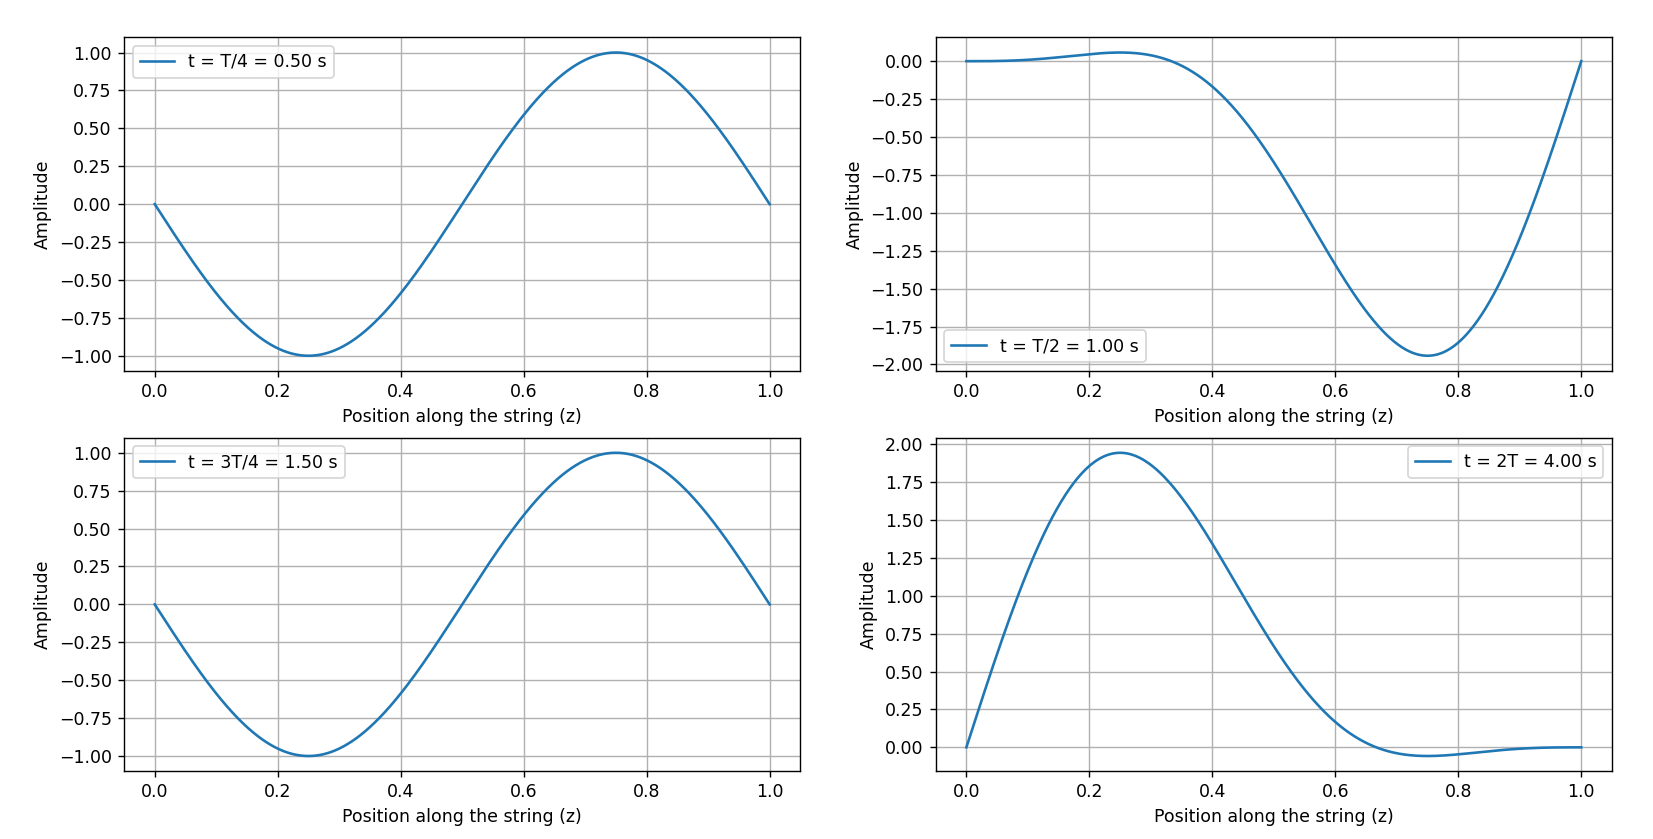
\includegraphics[width=0.919\textwidth]{Captura.PNG}
\end{figure}
\clearpage

\begin{figure}[h]
    \centering
    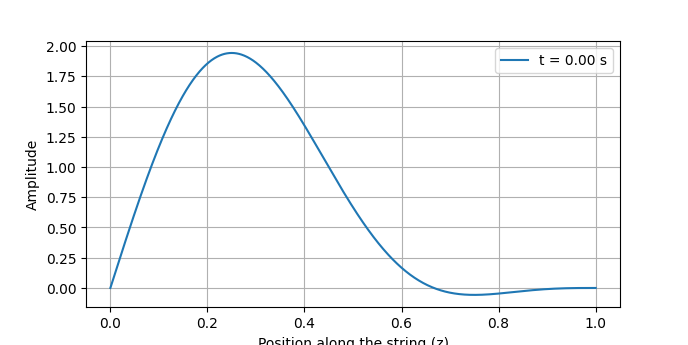
\includegraphics[width=0.55\textwidth]{t0.png}
\end{figure}

\begin{lstlisting}
import numpy as np
import matplotlib.pyplot as plt

# Constants
L = 1.0  # Length of the string
T1 = 2 * L  # Period of the lowest mode (fundamental frequency)
omega = [0, 2 * np.pi / T1, 2 * omega1, 3 * omega1]
z_values = np.linspace(0, L, 1000)
times = [0, T1 / 4, T1 / 2, 3 * T1 / 4, 2 * T1]

superposition_values = []
for t in times:
    superposition = (np.sin(np.pi * z_values) * np.cos(omega[1] * t)
        + np.sin(2 * np.pi * z_values) * np.cos(omega[2] * t)
        + (1 / 3) * np.sin(3 * np.pi * z_values) * np.cos(omega[3] * t))
    superposition_values.append(superposition)

# Plot the superposition at different times
plt.figure()
plt.plot(z_values, superposition_values[0], label=f"t = {times[0]:.2f} s")
plt.xlabel("Position along the string (z)")
plt.ylabel("Amplitude")
plt.legend()
plt.grid(True)

fig, axs = plt.subplots(2, 2)
axs[0, 0].plot(z_values, superposition_values[1], label=f"t = T/4 = {times[1]:.2f} s")
axs[0, 1].plot(z_values, superposition_values[2], label=f"t = T/2 = {times[2]:.2f} s")
axs[1, 0].plot(z_values, superposition_values[3], label=f"t = 3T/4 = {times[3]:.2f} s")
axs[1, 1].plot(z_values, superposition_values[4], label=f"t = 2T = {times[4]:.2f} s")
for ax in axs.flat:
    ax.set(xlabel='Position along the string (z)', ylabel='Amplitude')
    ax.grid(True)
    ax.legend()
plt.show()
\end{lstlisting}
\clearpage
\section*{Exercise 4}
\pregunta{
For a string with free ends at \(z = 0\) and \(z = L\), by using equation (8.30), show that the free end boundary at \(z = 0\) requires that \(C = 0\) in equation (8.16). Then use the boundary condition at \(z = L\) to derive the mode wavelengths. What are the mode frequencies?

Given equations:
\begin{itemize}
    \item Equation (8.30):  $\frac{dA(z)}{dz} = 0$
    \item Equation (8.16):  $A(z) = C\sin\left(\frac{2\pi z}{\lambda}\right) + D\cos\left(\frac{2\pi z}{\lambda}\right)$
\end{itemize}
}
\noindent First, we calculate the derivative of equation 8.16:
\[
\dfrac{dA}{dz}=-\dfrac{2{\pi}}{\lambda}\cdot\left(D\sin\left(\frac{2{\pi}z}{{\lambda}}\right)-C\cos\left(\frac{2{\pi}z}{{\lambda}}\right)\right)
\]
Since $sin(0)=0$, but $cos(0)\neq 0$, From equation (8.30), we find that \(C = 0\).
\[\dfrac{dA}{dz}(0)=0\Longleftrightarrow -\dfrac{2{\pi}}{\lambda}\cdot\left(D\sin\left(\frac{2{\pi}0}{{\lambda}}\right)-C\cos\left(\frac{2{\pi}0}{{\lambda}}\right)\right)=0\Longleftrightarrow C\cos (0) =0 \Longleftrightarrow C=0\]
\noindent Now let's use the boundary condition at \(z = L\) to derive the mode wavelengths:
\begin{align}
    A(L) &= D\cos\left(\frac{2\pi L}{\lambda}\right) = 0 \\
    \frac{2\pi L}{\lambda} &= n\pi \quad \text{(for nonzero solutions)} \\
    \lambda_n &= \frac{2L}{n}
\end{align}

\noindent The mode frequencies are related to the angular frequency:
\[ \omega_n = v k_n = \frac{n\pi v}{L} \]

\noindent The normal mode wavefunctions are:
\[ \Psi_n(z, t) = A_n \sin\left(\frac{n\pi z}{L}\right) \cos(\omega_n t) \]

\noindent Explicit formulas for \(\Psi_1(z, t)\) and \(\Psi_2(z, t)\):
\begin{align}
    \Psi_1(z, t) &= A_1 \sin\left(\frac{\pi z}{L}\right) \cos(\omega_1 t) \\
    \Psi_2(z, t) &= A_2 \sin\left(\frac{2\pi z}{L}\right) \cos(\omega_2 t)
\end{align}


\clearpage
\section*{Exercise 5}

An ideal stretched string of equilibrium linear mass density \(\rho l\) and equilibrium tension \(T_0\) has one free end at \(z = 0\) and one bound end at \(z = L\).
\subsection*{Part a}
\pregunta{
\begin{enumerate}
    \item Draw sketches of the two lowest nonzero frequency normal mode shapes on this string (no derivation necessary). As part of your drawings, be sure to show the “equilibrium line” for the string.
    \item From simple observation of your sketches, state clearly the wavelength of each of these two normal modes. Extrapolating your results, are the mode frequencies all integer harmonics of the frequency of the lowest normal mode? Are some integer harmonics of the fundamental “missing”? If so, which?
\end{enumerate}}

\noindent Here are the sketches of the two lowest nonzero frequency normal modes for the stretched string:
\begin{figure}[h]
    \centering
    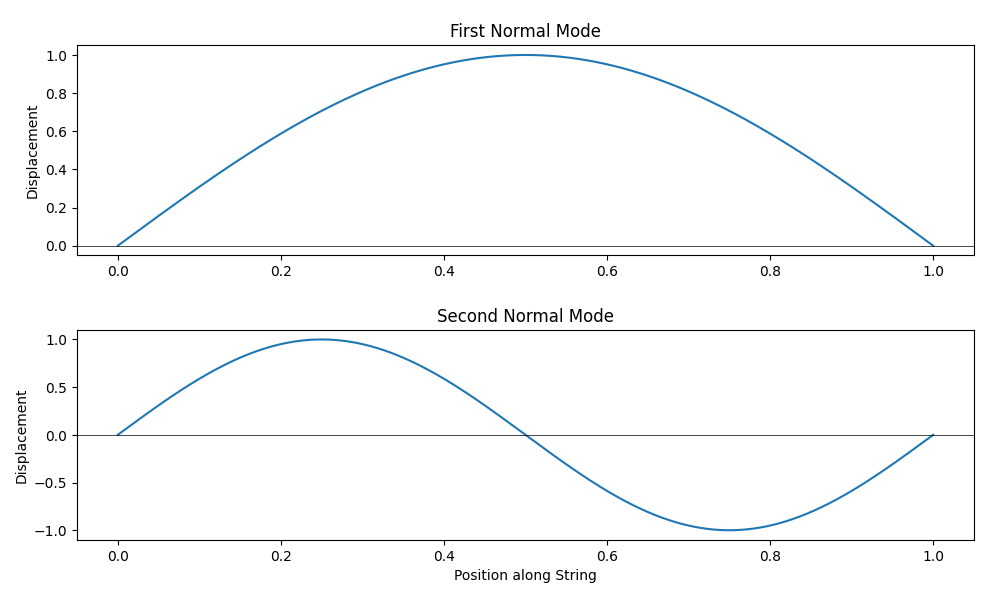
\includegraphics[width=0.7\textwidth]{Figure_1.png}
\end{figure}

\subsubsection*{First Normal (Fundamental) Mode:}
The string vibrates with a single antinode (maximum displacement) at the midpoint (\(z = \frac{L}{2}\)). The equilibrium line (no displacement) is a straight line connecting the free end (\(z = 0\)) and the bound end (\(z = L\)). The wavelength of this mode is twice the length of the string: \(\lambda_1 = 2L\).

\subsubsection*{Second Normal Mode:}
    The string vibrates with two antinodes (maximum displacements) at equal distances from the midpoint (\(z = \frac{L}{2}\)). The equilibrium line remains the same as in the first mode. The wavelength of this mode is half the length of the string: \(\lambda_2 = L\).

\subsubsection*{Observations and Extrapolation}
    The mode frequencies are not all integer harmonics of the fundamental frequency. Some integer harmonics of the fundamental are missing. Specifically, the second harmonic (twice the fundamental frequency) is missing.

\subsection*{Part b}
\pregunta{
Derive the allowed normal mode wavelengths and the normal mode wavefunction \(\Psi_n(z,t)\) for “normal mode \(n\)” on this string.\\

\noindent Your derivation must start with the appropriate form of the general solution of the Helmholtz equation. Then, applying the boundary conditions (state them explicitly), derive mathematically in a step-by-step fashion:
\begin{enumerate}
    \item The mode wavelengths.
    \item The mode frequencies.
    \item The normal mode wavefunctions \(\Psi_n(z,t)\).
\end{enumerate}

From your final result, write out explicitly the formula for each of \(\Psi_1(z,t)\) and \(\Psi_2(z,t)\).}

The general solution for the transverse wave on a stretched string is given by:
\[ \Psi(z, t) = A_n \sin(k_n z) \cos(\omega_n t) \]

Where:
\begin{itemize}
    \item \(A_n\) is the amplitude of the normal mode.
    \item \(k_n\) is the wave number associated with the mode.
    \item \(\omega_n\) is the angular frequency of the mode.
\end{itemize}

\subsection*{Boundary Conditions}

\subsubsection*{Free End (\(z = 0\)):}
The displacement at the free end is zero: \(\Psi(0, t) = 0\). This gives us: \(A_n \sin(0) = 0\), which implies that \(A_n = 0\) for all modes.

\subsubsection*{Bound End (\(z = L\)):}
The displacement at the bound end is zero: \(\Psi(L, t) = 0\). This gives us: \(A_n \sin(k_n L) = 0\). For nonzero solutions, we require: \(k_n L = n\pi\), where \(n\) is a positive integer.

\subsection*{Deriving Normal Mode Properties}

\begin{enumerate}
    \item \textbf{Mode Wavelengths}:
    From the boundary condition: \(k_n L = n\pi\), solving for \(k_n\):
    \[ k_n = \frac{n\pi}{L} \]
    The mode wavelengths are:
    \[ \lambda_n = \frac{2\pi}{k_n} = \frac{2L}{n} \]

    \item \textbf{Mode Frequencies}:
    The mode frequencies are related to the angular frequency:
    \[ \omega_n = v k_n = \frac{n\pi v}{L} \]
    where \(v\) is the wave speed on the string.

    \item \textbf{Normal Mode Wavefunctions}:
    The normal mode wavefunction is:
    \[ \Psi_n(z, t) = A_n \sin\left(\frac{n\pi z}{L}\right) \cos(\omega_n t) \]

    \item \textbf{Explicit Formulas for \(\Psi_1(z, t)\) and \(\Psi_2(z, t)\)}:
    \begin{itemize}
        \item First Normal Mode (Fundamental Mode):
        \[ \Psi_1(z, t) = A_1 \sin\left(\frac{\pi z}{L}\right) \cos(\omega_1 t) \]

        \item Second Normal Mode:
        \[ \Psi_2(z, t) = A_2 \sin\left(\frac{2\pi z}{L}\right) \cos(\omega_2 t) \]
    \end{itemize}
\end{enumerate}

I should note that the mode frequencies \(\omega_n\) are proportional to the wave speed on the string. The missing second harmonic corresponds to the absence of the second mode frequency.



\end{document}


